\subsection{Shape Module: Generating a Shape Descriptor}
\label{sec:architecture-shape-module}
The objective of the shape module is combining the group descriptors to a single shape descriptor that can be used for the classification.
This descriptor contains every important feature of all views and groups.
As usual, the tensor $\bar{\vec{G}}$ containing all the group descriptors of every batch is processed by each batch element.
This batch element $\vec{G}$ of size $n_v \times 6 \times 6 \times 256$ contains the $n_v$ group descriptors of an object.
This tensor is split across its first dimension, i.d. across the group descriptors, resulting in a tensor for each group descriptor.
Each group descriptor is then fed into a fully-connected sub-network with two layers.
The first layer has $6\cdot6\cdot256$ edges per unit and 4096 units in total, while the second layer has 4069 edges per unit and 4069 output units as well.
The inputs are processed like in the fully-connected layer before.
First, each input $\vec{G}_g$ is flattened into a column-vector $\vec{g}_g$.
Then, a matrix multiplication of the inputs and the corresponding weight matrix is performed and a bias vector is added.
This result is fed into a ReLU activation function $\phi(\cdot)$ resulting in an activation for the particular layer.
In conclusion, the two fully-connected operations
\begin{subequations}
	\begin{align}
		\vec{a}^{[6]}_g &= \phi(\vec{W}^{[6]} \vec{g}_g + \vec{b}^{[6]}) \\
		\vec{a}^{[7]}_g &= \phi(\vec{W}^{[7]} \vec{a}^{[7]}_g + \vec{b}^{[7]})
	\end{align}
\end{subequations}
are performed as illustrated in \figref{fig:shape-module-group-shape}.
\begin{figure}
	\centering
	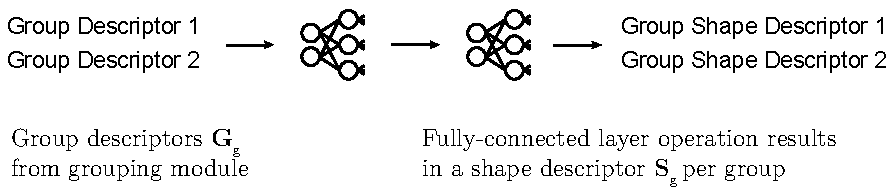
\includegraphics[]{images/shape_module_group_shape.pdf}
	\caption[Generate group shape descriptors in shape module]{Generate group shape descriptors in shape module. Each group descriptor is fed into two fully-connected layers representing layer 6 and 7 of the network. The activation of layer 7 represents the shape descriptor of each group descriptor.}
	\label{fig:shape-module-group-shape}
\end{figure}
Furthermore, both layers contain a dropout layer with a dropout probability of $0.5$.
This corresponds to the original AlexNet configuration.
Hence, the final activations of the seventh layer in the network or second dense layer, respectively, represent the shape descriptor of every group descriptor.
Those single shape descriptor vectors of each group are then again stacked along the first dimension for having a compact representation $\vec{S}_g$ with size $n_v \times 4096$.
Expanding this with a batch dimension yields the tensor $\bar{\vec{S}_g}$ with size $Batch \times n_v \times 4096$.

Now the group shape descriptors need to be combined for generating the final single shape descriptor of the object.
This is done by considering the group weights $\vec{w}$ with $n_v$ elements calculated in the grouping module.
As a reminder, they are the mean of all view scores of each group and, thus, an indicator for the group's discrimination.
Hence, a weighted average is calculated for considering this relation.
For having a valid matrix multiplication, the group shape descriptor $\bar{\vec{S}_g}$ needs to be transposed while keeping the batch dimension as the first one.
Hence its size changes from $Batch \times n_v \times 4096$ to $Batch \times 4096 \times n_v$.
Furthermore, the group weights tensor $\bar{\vec{W}}_g$ is expanded with a third dimension yielding the shape $Batch \times n_v \times 1$.
For this weighted average calculation a tensor holding the sums of the weights in inevitable.
Thus, $\bar{\vec{W}}_{g,\text{sum}}$ stores the sum of the group weights tensor along its first dimension, i.e. each element is the sum of all group weights of an object.
For a valid matrix division, a third dimension must be expanded as well.
This yields a tensor $\bar{\vec{W}}_{g,\text{sum}}$ of the shape $Batch \times 1 \times 1$ with weight sums.
Now the weighted average can be computed by
\begin{equation}
	\vec{S} = \frac{\vec{S}_g \vec{W}_g} {\vec{W}_{g,\text{sum}}}
\end{equation}
where the division is performed element-wise.
Due to the matrix multiplication, the padded entries have no impact.
The result of the assembled tensor $\bar{\vec{S}}$ has a shape of $Batch \times 4096 \times 1$ and represents the final single shape descriptor.
This can be made more compact by changing the shape to $Batch \times 4096$ without losing any information because the number of elements stays the same.

This representation is directly compatible with the last fully-connected layer, which is responsible for calculating the predictions of the network, thus, $\bar{\vec{S}}$ is fed into it.
The number of neurons in this layer equals the number of different labels or categories, respectively, where each neuron has 4096 edges.
The performed operations are identical to the ones earlier and are described by
\begin{equation}
	\vec{z}^{[8]} = \vec{W}^{[8]} \vec{S} + \vec{b}^{[8]}
\end{equation}
using the related weights and biases.
However, no activation function is applied here.
For making the predictions $\vec{z}^{[8]}$ interpretable, they are fed into a softmax layer.
This outputs a valid probability distribution $\hat{\vec{y}}$ depending on all its inputs $\vec{z}^{[8]}$.
Hence, this results in a membership probability for the network's input to each class.
The class representing the index with the largest value in $\hat{\vec{y}}$ is considered the predicted class. The functionality of the shape module is summarized in \figref{fig:shape-module-final-shape}.
\begin{figure}
	\centering
	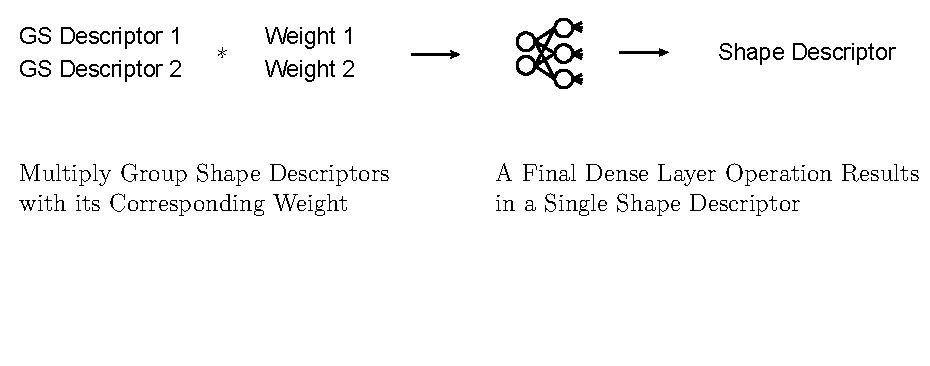
\includegraphics[]{images/shape_module_final_shape.pdf}
	\caption[Basic concept of the shape module]{Basic concept of the shape module combined with a classification. A weighted average of the group shape descriptors with the related group weights is calculated yielding a single shape descriptor. It is fed into the last fully-connected layer resulting in the prediction of the network.}
	\label{fig:shape-module-final-shape}
\end{figure}